%!TEX TS-program = xelatex

% Шаблон документа LaTeX создан в 2018 году
% Алексеем Подчезерцевым
% В качестве исходных использованы шаблоны
% 	Данилом Фёдоровых (danil@fedorovykh.ru) 
%		https://www.writelatex.com/coursera/latex/5.2.2
%	LaTeX-шаблон для русской кандидатской диссертации и её автореферата.
%		https://github.com/AndreyAkinshin/Russian-Phd-LaTeX-Dissertation-Template

\documentclass[a4paper,14pt]{article}


%%% Работа с русским языком
\usepackage[english,russian]{babel}   %% загружает пакет многоязыковой вёрстки
\usepackage{fontspec}      %% подготавливает загрузку шрифтов Open Type, True Type и др.
\defaultfontfeatures{Ligatures={TeX},Renderer=Basic}  %% свойства шрифтов по умолчанию
\setmainfont[Ligatures={TeX,Historic}]{Times New Roman} %% задаёт основной шрифт документа
\setsansfont{Comic Sans MS}                    %% задаёт шрифт без засечек
\setmonofont{Courier New}
\usepackage{indentfirst}
\frenchspacing

\renewcommand{\epsilon}{\ensuremath{\varepsilon}}
\renewcommand{\phi}{\ensuremath{\varphi}}
\renewcommand{\kappa}{\ensuremath{\varkappa}}
\renewcommand{\le}{\ensuremath{\leqslant}}
\renewcommand{\leq}{\ensuremath{\leqslant}}
\renewcommand{\ge}{\ensuremath{\geqslant}}
\renewcommand{\geq}{\ensuremath{\geqslant}}
\renewcommand{\emptyset}{\varnothing}

%%% Дополнительная работа с математикой
\usepackage{amsmath,amsfonts,amssymb,amsthm,mathtools} % AMS
\usepackage{icomma} % "Умная" запятая: $0,2$ --- число, $0, 2$ --- перечисление

%% Номера формул
%\mathtoolsset{showonlyrefs=true} % Показывать номера только у тех формул, на которые есть \eqref{} в тексте.
%\usepackage{leqno} % Нумерация формул слева	

%% Перенос знаков в формулах (по Львовскому)
\newcommand*{\hm}[1]{#1\nobreak\discretionary{}
	{\hbox{$\mathsurround=0pt #1$}}{}}

%%% Работа с картинками
\usepackage{graphicx}  % Для вставки рисунков
\graphicspath{{images/}}  % папки с картинками
\setlength\fboxsep{3pt} % Отступ рамки \fbox{} от рисунка
\setlength\fboxrule{1pt} % Толщина линий рамки \fbox{}
\usepackage{wrapfig} % Обтекание рисунков текстом

%%% Работа с таблицами
\usepackage{array,tabularx,tabulary,booktabs} % Дополнительная работа с таблицами
\usepackage{longtable}  % Длинные таблицы
\usepackage{multirow} % Слияние строк в таблице
\usepackage{float}% http://ctan.org/pkg/float

%%% Программирование
\usepackage{etoolbox} % логические операторы


%%% Страница
\usepackage{extsizes} % Возможность сделать 14-й шрифт
\usepackage{geometry} % Простой способ задавать поля
\geometry{top=20mm}
\geometry{bottom=20mm}
\geometry{left=20mm}
\geometry{right=10mm}
%
%\usepackage{fancyhdr} % Колонтитулы
% 	\pagestyle{fancy}
%\renewcommand{\headrulewidth}{0pt}  % Толщина линейки, отчеркивающей верхний колонтитул
% 	\lfoot{Нижний левый}
% 	\rfoot{Нижний правый}
% 	\rhead{Верхний правый}
% 	\chead{Верхний в центре}
% 	\lhead{Верхний левый}
%	\cfoot{Нижний в центре} % По умолчанию здесь номер страницы

\usepackage{setspace} % Интерлиньяж
\onehalfspacing % Интерлиньяж 1.5
%\doublespacing % Интерлиньяж 2
%\singlespacing % Интерлиньяж 1

\usepackage{lastpage} % Узнать, сколько всего страниц в документе.

\usepackage{soul} % Модификаторы начертания

\usepackage{hyperref}
\usepackage[usenames,dvipsnames,svgnames,table,rgb]{xcolor}
\hypersetup{				% Гиперссылки
	unicode=true,           % русские буквы в раздела PDF
	pdftitle={Заголовок},   % Заголовок
	pdfauthor={Автор},      % Автор
	pdfsubject={Тема},      % Тема
	pdfcreator={Создатель}, % Создатель
	pdfproducer={Производитель}, % Производитель
	pdfkeywords={keyword1} {key2} {key3}, % Ключевые слова
	colorlinks=true,       	% false: ссылки в рамках; true: цветные ссылки
	linkcolor=black,          % внутренние ссылки
	citecolor=black,        % на библиографию
	filecolor=magenta,      % на файлы
	urlcolor=black           % на URL
}
\makeatletter 
\def\@biblabel#1{#1. } 
\makeatother
\usepackage{cite} % Работа с библиографией
%\usepackage[superscript]{cite} % Ссылки в верхних индексах
%\usepackage[nocompress]{cite} % 
\usepackage{csquotes} % Еще инструменты для ссылок

\usepackage{multicol} % Несколько колонок

\usepackage{tikz} % Работа с графикой
\usepackage{pgfplots}
\usepackage{pgfplotstable}

% ГОСТ заголовки
\usepackage[font=small]{caption}
%\captionsetup[table]{justification=centering, labelsep = newline} % Таблицы по правобу краю
%\captionsetup[figure]{justification=centering} % Картинки по центру


\newcommand{\tablecaption}[1]{\addtocounter{table}{1}\small \begin{flushright}\tablename \ \thetable\end{flushright}%	
\begin{center}#1\end{center}}

\newcommand{\imref}[1]{рис.~\ref{#1}}

\usepackage{multirow}
\usepackage{spreadtab}
\newcolumntype{K}[1]{@{}>{\centering\arraybackslash}p{#1cm}@{}}


\usepackage{xparse}
\usepackage{fancyvrb}

\RecustomVerbatimCommand{\VerbatimInput}{VerbatimInput}
{
	fontsize=\footnotesize    
}

\usepackage{tocloft}
\renewcommand{\cftsecleader}{\cftdotfill{\cftdotsep}}
\begin{document} % конец преамбулы, начало документа
\begin{titlepage}
	\begin{center}
 		ФЕДЕРАЛЬНОЕ  ГОСУДАРСТВЕННОЕ АВТОНОМНОЕ \\
		ОБРАЗОВАТЕЛЬНОЕ УЧРЕЖДЕНИЕ ВЫСШЕГО ОБРАЗОВАНИЯ\\
		«НАЦИОНАЛЬНЫЙ ИССЛЕДОВАТЕЛЬСКИЙ УНИВЕРСИТЕТ\\
		«ВЫСШАЯ ШКОЛА ЭКОНОМИКИ»
	\end{center}
	
	\begin{center}
		\textbf{Московский институт электроники и математики}
		
		\textbf{им. А.Н.Тихонова НИУ ВШЭ}
		
		\vspace{2ex}
		
		\textbf{Департамент компьютерной инженерии}
	\end{center}
	\vspace{1ex}	
	
	\begin{center}
	\textbf{ОТЧЕТ\\
		ПО ЛАБОРАТОРНОЙ РАБОТЕ №6
	}
	\end{center}	
	\vspace{2ex}
	\begin{center}
		по дисциплине «Проектирование систем на кристалле»
	\end{center}	

	\vspace{2ex}

	\begin{flushright}
		\textbf{Выполнили:}
		
		\vspace{2ex}
		
		Студенты группы БИВ174
		
		Бригада №5
		
		\vspace{2ex}
		
		Подчезерцев Алексей Евгеньевич
		
		Солодянкин Андрей Александрович
		\vspace{2ex}
		
	\end{flushright}

	\vfill
	\begin{center}
		Москва \the\year \, г.
	\end{center}
	
\end{titlepage}
\addtocounter{page}{1}
\tableofcontents
\pagebreak

\section{Задание}

Опишите идею прикладного программно-аппаратного проекта с использованием ПЛИС или одноплатного компьютера.

\section{Идея проекта}

Трекинг позиции окончания пишущего устройства на бумаге для непрерывной оцифровки рукописи человека.
В условиях удаленного обучения часть студентов испытывает трудности с выступлением у виртуальной <<доски>>, так как они не могут с той же скоростью и качеством писать что-либо с помощью устройства позиционирования курсора операционной системы. Данная проблема тратит время преподавателя на семинарах и других типах занятий, студентов, которые наблюдают за занятием, непосредственно выступающего учащегося.
Данное решение позволит экономить время всех участников и не тратить большие финансовые вложения в графические планшеты, которые могут и не пригодиться в будущем.

\section{Заказчик проекта}

Потенциальные заказчики -- Московский институт электроники и математики им. А.Н. Тихонова, коммерческая компания, стартап.

\section{Потребитель проекта}

Студенты; люди, не имеющие возможности приобрести графический планшет ввиду его большой стоимости и крайнего узкого спектра применения.

\section{Польза проекта}

Проект позволяет в реальном времени отслеживает движение пишущего устройства (ручки, карандаша и других канцелярский принадлежностей) по поверхности бумаги и оцифровывает полученные кривые в пригодный для отображения на персональном компьютере.
В отличии от графического планшета стоимость устройства должна быть заметно ниже.
В отличии от устройств позиционирования курсора для персонального компьютера, которые не позволяют быстро и качественно отображать формулы и другую графическую информацию, данное устройство позволит выводить информацию, которая создается естественным путем -- написанием от руки.

\section{Схема проекта}

Схема проекта представлена на рис.~\ref{fig:schema}.
Камера осуществляет захват изображения и передает его на одноплатный компьютер или ПЛИС.
Последнее устройство осуществляет обработку видеоинформации, занимается поиском нужных объектов на видеоизображении и строит распознанные кривые.
Полученные данные передаются на персональный компьютер или мобильное устройство пользователя посредством проводного или беспроводного протокола передачи данных в виде векторного или растрового изображения или в виде команд для устройства позиционирования указателя операционной системы пользователя -- курсора.

\begin{figure}[H]
	\centering
	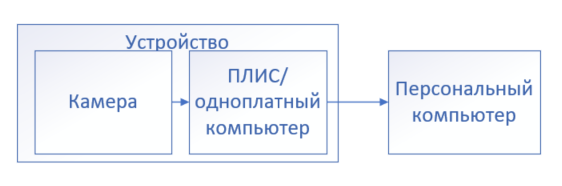
\includegraphics[width=\linewidth]{image/schema}
	\caption{Схема проекта}
	\label{fig:schema}
\end{figure}

\section{Составляющие проекта}

Первая составляющая проекта, которая выполняет захват изображения -- камера.
Следующая составляющая проекта -- ПЛИС или одноплатный компьютер.
Данное устройство выполняет обработку видеоинформации, осуществляет поиск необходимых объектов на видеоизображении и строит итоговые кривые.
Передача данных между данными устройствами осуществляется по протоколу камеры (USB, Wi-Fi, etc.).

Передача данных от устройства выполняется путем использования протоколов проводной передачи данных (USB) или беспроводной передачи данных: Wi-Fi, Bluetooth.
Конечное решение принимает команда разработки в зависимости от сложности, стоимости и удобства использования того или иного протокола.

\section{Шаги проекта}

Для успешной реализации проекта необходимо пройти следующие этапы:

\begin{itemize}
	\item Разработка программного прототипа.

	На данном этапе необходимо подтвердить работоспособность идеи отслеживания позиции пишущего устройства, оценить затраты на вычислительные ресурсы и качество получаемого решения.
	Одновременно необходимо выбрать оборудование для захвата видеоряда и собрать видеозаписи, на которых будет проверяться качество полученного алгоритма.
	
	\item Выбор одноплатного компьютера или ПЛИС и перенос кода.
	
	На данном этапе необходимо выбрать устройство, которое способно обрабатывать видеоряд в реальном времени в соответствии с затратами алгоритма и его реализацией в коде на данном устройстве.
	
	\item Создание финального прототипа.
	
	На данном этапе команда проекта создает дизайн внешнего вида устройства и оформляет как законченный продукт. 
	Также проходит тестирование устройства на соответствие поставленным задачам и получаемым результатам.
	
	\item Демонстрация проекта, серийное производство.
	
	Команда проекта демонстрирует полученные результаты, занимается поиском возможных инвесторов, готовится в массовому производству.
	
\end{itemize}

\section{Аппаратная платформа проекта}

В качестве аппаратной платформы используется De10-Nano или другой ПЛИС, или Raspberry Pi 4 или другой одноплатный компьютер или устройство другой архитектуры, в зависимости от требований проекта, например мобильные устройства или вычислительные системы архитектуры x86.
В качестве камеры используется устройство с разрешением не менее 1280x720 и совместимым с выбранной аппаратной платформой.

\section{Затраты проекта}

Список затрат проекта (без учета оплаты труда команды разработчиков) представлен на таблице~\ref{tab:my-table}.
На первом этапе основной источник затрат -- камера, а также запись датасетов для обучения алгоритмов.
На следующем этапе потребуются финансы для тестирования алгоритмов на выбранном железе.
При создании финального прототипа потребуется создание корпуса и демонстрационных материалов; оплаты труда тестировщиков полученного устройства.
На финальном этапе трудно оценить затраты, но часть из них может пойти на доработку системы, создания большего числа прототипов, рекламу и другие цели.

\begin{table}[H]
	\caption{Список затрат на каждый этап проекта}
	\label{tab:my-table}
	\begin{tabular}{|c|c|c|}
		\hline
		Этап                 & Временные затраты, мес & Финансовые затраты, 1000₽ \\ \hline
		Разработка прототипа & 2-3                    & 10                        \\ \hline
		Выбор платформы      & 1-2                    & 30                        \\ \hline
		Финальный прототип   & 0,5-1                  & 20                        \\ \hline
		Демо                 & 3+                     & 50+                       \\ \hline
	\end{tabular}
\end{table}

\end{document} % конец документа